\documentclass[11pt,letterpaper]{article}

\usepackage[margin=1in]{geometry}
\usepackage{setspace}
\onehalfspacing

\usepackage{microtype}
\usepackage{booktabs}
\usepackage{longtable}
\usepackage{array}
\usepackage{tabularx}
\usepackage{xcolor}
\usepackage{amsmath,amssymb}
\usepackage{tikz}
\usetikzlibrary{shapes.geometric, arrows.meta, positioning, fit, backgrounds, calc}
\usepackage[hyphens]{url}
\usepackage[colorlinks=true,linkcolor=blue,citecolor=blue,urlcolor=blue]{hyperref}
\usepackage{cleveref}
\usepackage[numbers,sort&compress]{natbib}
\usepackage{enumitem}

\title{
    \vspace{-1cm}
    \textbf{Update 15: Architecture Comparison---Autoregressive, Diffusion, and State Space Models} \\[0.5em]
    \large KV Cache Strategies, Time Complexity, and Inference Benchmarking with vLLM
}

\author{
    Nathan Gopee \\
    \textit{MS Computer Science Candidate} \\
    SUNY New Paltz \\
    \texttt{gopeen1@newpaltz.edu}
}

\date{February 2026}

\begin{document}

\maketitle

\begin{abstract}
\noindent
This update compares three fundamentally different language model architectures---autoregressive Transformers (GPT-oss via vLLM~\cite{vllm,gptoss}), discrete diffusion models (MDLM~\cite{mdlm}, SEDD~\cite{sedd}), and selective state space models (Mamba/Granite~4~\cite{mamba,granite})---with emphasis on how each handles inference state (KV cache vs.\ recurrent state vs.\ iterative denoising), time complexity scaling, and practical throughput on consumer GPU hardware. We derive the per-token and total generation cost for each paradigm, compare memory scaling with sequence length, and present a benchmarking plan for the lab cluster (RTX~3090, RTX~5090, Tesla~V100).
\end{abstract}

%=============================================================================
\section{Three Paradigms for Language Model Inference}
%=============================================================================

Modern language models fall into three architectural families, each with distinct inference characteristics:

\begin{enumerate}[noitemsep]
    \item \textbf{Autoregressive Transformers}: Generate tokens left-to-right, one per forward pass. Each step attends to all prior tokens via a KV cache that grows linearly with context. Examples: GPT-4, Llama, GPT-oss~\cite{gptoss}.

    \item \textbf{Diffusion Language Models}: Start with a fully masked or noised sequence and iteratively denoise all tokens in parallel over $T$ refinement steps ($T \ll n$). No KV cache; each step recomputes full bidirectional attention. Examples: MDLM~\cite{mdlm}, SEDD~\cite{sedd}, Mercury~\cite{mercury}.

    \item \textbf{State Space Models (SSMs)}: Process tokens sequentially through a fixed-size recurrent state that compresses all history into $O(d \cdot N)$ values per layer, independent of sequence length. No KV cache. Examples: Mamba~\cite{mamba}, Mamba-2~\cite{mamba2}, Granite~4~\cite{granite}.
\end{enumerate}

\begin{figure}[htbp]
\centering
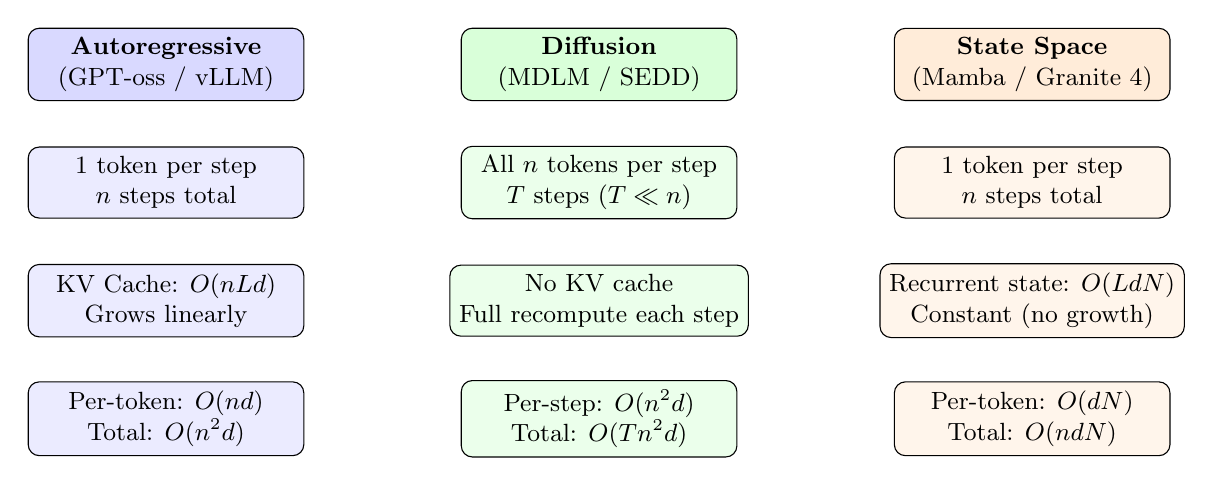
\begin{tikzpicture}[
    node distance=0.8cm,
    box/.style={rectangle, draw, rounded corners, minimum width=3.5cm, minimum height=0.8cm, align=center, font=\small},
    arrow/.style={->, thick, >=Stealth}
]
    % AR column
    \node[box, fill=blue!15] (ar-title) at (0,0) {\textbf{Autoregressive}\\(GPT-oss / vLLM)};
    \node[box, fill=blue!8] (ar-step) at (0,-1.5) {1 token per step\\$n$ steps total};
    \node[box, fill=blue!8] (ar-cache) at (0,-3.0) {KV Cache: $O(nLd)$\\Grows linearly};
    \node[box, fill=blue!8] (ar-cost) at (0,-4.5) {Per-token: $O(nd)$\\Total: $O(n^2 d)$};

    % Diffusion column
    \node[box, fill=green!15] (diff-title) at (5.5,0) {\textbf{Diffusion}\\(MDLM / SEDD)};
    \node[box, fill=green!8] (diff-step) at (5.5,-1.5) {All $n$ tokens per step\\$T$ steps ($T \ll n$)};
    \node[box, fill=green!8] (diff-cache) at (5.5,-3.0) {No KV cache\\Full recompute each step};
    \node[box, fill=green!8] (diff-cost) at (5.5,-4.5) {Per-step: $O(n^2 d)$\\Total: $O(Tn^2 d)$};

    % Mamba column
    \node[box, fill=orange!15] (ssm-title) at (11,0) {\textbf{State Space}\\(Mamba / Granite 4)};
    \node[box, fill=orange!8] (ssm-step) at (11,-1.5) {1 token per step\\$n$ steps total};
    \node[box, fill=orange!8] (ssm-cache) at (11,-3.0) {Recurrent state: $O(LdN)$\\Constant (no growth)};
    \node[box, fill=orange!8] (ssm-cost) at (11,-4.5) {Per-token: $O(dN)$\\Total: $O(ndN)$};
\end{tikzpicture}
\caption{Comparison of inference characteristics across three architecture paradigms. $n$=sequence length, $d$=model dimension, $L$=layers, $N$=SSM state dimension (typically 16), $T$=diffusion steps (typically 32--256).}
\label{fig:paradigms}
\end{figure}

%=============================================================================
\section{Autoregressive Transformers: GPT-oss via vLLM}
\label{sec:autoregressive}
%=============================================================================

\subsection{GPT-oss Architecture}

GPT-oss-120b~\cite{gptoss} is an open-source Mixture-of-Experts (MoE) model with 116.8~billion total parameters. Using MXFP4 quantization, the model compresses to approximately 63~GB, enabling deployment across consumer GPUs via tensor parallelism in vLLM~\cite{vllm}. The MoE architecture routes each token to a subset of expert FFN blocks (top-2 out of 16 experts), so the active parameter count per token is substantially lower than the total.

\subsection{KV Cache in Autoregressive Models}

The KV cache stores the key and value projections from all prior tokens at every attention layer, enabling each new token to attend to the full context without recomputing all past representations.

For a model with $L$ layers, $H_{kv}$ KV heads (under Grouped Query Attention), and head dimension $d_k$:

\begin{equation}
    \text{KV cache size} = 2 \cdot L \cdot H_{kv} \cdot d_k \cdot n \cdot b
    \label{eq:kv-cache}
\end{equation}

where $n$ is the current sequence length and $b$ is the bytes per element (2 for FP16). For a 7B-class model ($L=32$, $H_{kv}=8$, $d_k=128$):

\begin{table}[htbp]
\centering
\caption{KV cache memory scaling for a 7B-class Transformer}
\label{tab:kv-scaling}
\begin{tabular}{@{}rrrr@{}}
\toprule
\textbf{Context Length} & \textbf{KV Cache} & \textbf{Per-Token Cost} & \textbf{Attention FLOPs/token} \\
\midrule
512 & 64 MB & 128 KB & $6.7 \times 10^7$ \\
2,048 & 256 MB & 128 KB & $2.7 \times 10^8$ \\
8,192 & 1 GB & 128 KB & $1.1 \times 10^9$ \\
32,768 & 4 GB & 128 KB & $4.3 \times 10^9$ \\
131,072 & 16 GB & 128 KB & $1.7 \times 10^{10}$ \\
\bottomrule
\end{tabular}
\end{table}

The per-token KV cache addition is constant (128~KB), but the attention computation grows linearly because each new token must attend to all cached keys. At 128K context, the KV cache alone consumes 16~GB---a significant fraction of an RTX~3090's 24~GB VRAM.

\subsection{vLLM PagedAttention}

vLLM~\cite{vllm} addresses KV cache fragmentation via PagedAttention, which stores KV blocks in non-contiguous GPU memory pages (analogous to virtual memory). This eliminates internal fragmentation and enables dynamic batching of requests with different context lengths. For the RDMA middleware, PagedAttention's block-granular KV management maps naturally to RDMA scatter/gather operations for disaggregated prefill-decode serving.

\subsection{Time Complexity}

\begin{itemize}[noitemsep]
    \item \textbf{Prefill} (processing prompt of length $p$): $O(L \cdot p^2 \cdot d)$ for self-attention across the prompt. Parallelizable across the $p$ tokens.
    \item \textbf{Per-token generation}: $O(L \cdot (n \cdot d + d^2))$ where $n$ is the current context. The $n \cdot d$ term (attention against KV cache) dominates at long contexts. The $d^2$ term (FFN) is constant.
    \item \textbf{Total generation} of $n$ tokens: $O(L \cdot n^2 \cdot d)$ because attention cost sums as $1 + 2 + \cdots + n = n(n+1)/2$.
\end{itemize}

\paragraph{Practical throughput.}
On a single RTX~3090 (24~GB), a 7B model in FP16 generates ${\sim}30$--50 tokens/sec at short context ($<$4K) but degrades to ${\sim}10$--15 tokens/sec at 128K context as the KV cache fills VRAM and attention becomes memory-bandwidth bound. vLLM's continuous batching mitigates this for concurrent requests.

%=============================================================================
\section{Diffusion Language Models: MDLM and SEDD}
\label{sec:diffusion}
%=============================================================================

\subsection{Discrete Diffusion for Text}

Unlike image diffusion (which operates in continuous pixel/latent space), text diffusion must handle a discrete vocabulary. Two dominant approaches have emerged:

\begin{itemize}[noitemsep]
    \item \textbf{Absorbing-state / Masked diffusion}: Tokens are progressively replaced with a \texttt{[MASK]} token during the forward process. The reverse process learns to unmask them. This connects directly to masked language modeling (BERT). Used by MDLM~\cite{mdlm} and D3PM~\cite{d3pm} (absorbing variant).

    \item \textbf{Score-based discrete diffusion}: Rather than predicting masked tokens, the model learns probability ratios (``concrete scores'') for transitioning between discrete states. Used by SEDD~\cite{sedd}.
\end{itemize}

\subsection{MDLM: Masked Diffusion Language Models}

MDLM~\cite{mdlm} (Sahoo et al., NeurIPS 2024) simplifies discrete diffusion by casting it as time-weighted masked language modeling. The forward process masks tokens according to a schedule $\alpha(t)$, and the training loss reduces to:

\begin{equation}
    \mathcal{L} = \mathbb{E}_{t, x_0} \left[ \frac{-\alpha'(t)}{\alpha(t)} \sum_{i: x_t^i = \texttt{[M]}} \log p_\theta(x_0^i \mid x_t, t) \right]
    \label{eq:mdlm-loss}
\end{equation}

where $\alpha(t) = (1-t)^{1/s}$ is a geometric noise schedule with learned exponent $s$. At GPT-2 scale (${\sim}110$M parameters), MDLM achieves perplexity of ${\sim}27.2$ on OpenWebText, slightly outperforming GPT-2 small (${\sim}29.4$ perplexity).

\subsection{SEDD: Score Entropy Discrete Diffusion}

SEDD~\cite{sedd} (Lou, Meng, Ermon; ICML 2024) parameterizes the ``concrete score''---the ratio of transition probabilities in discrete diffusion:

\begin{equation}
    s_\theta(x_t, t)[i, j] = \frac{p_\theta(x_0 = j \mid x_t, t)}{p_\theta(x_0 = x_t^i \mid x_t, t)}
    \label{eq:sedd-score}
\end{equation}

This avoids computing intractable normalizing constants. SEDD achieves ${\sim}31.4$ perplexity on OpenWebText at GPT-2 scale and establishes the theoretical foundations that led to Mercury~\cite{mercury}, the first commercially deployed diffusion LLM (developed by Inception Labs, co-founded by SEDD author Aaron Lou and Stefano Ermon).

\subsection{No KV Cache---Full Recompute Each Step}

Diffusion LLMs use \textbf{bidirectional attention} (no causal mask) because all tokens are visible at every denoising step. This means:

\begin{itemize}[noitemsep]
    \item No KV cache accumulation between generation steps---each of the $T$ diffusion steps performs a complete forward pass over the full $n$-token sequence.
    \item Each step costs $O(L \cdot n^2 \cdot d)$ for full bidirectional self-attention.
    \item Total generation: $O(T \cdot L \cdot n^2 \cdot d)$ where $T$ is the number of denoising steps.
\end{itemize}

The total FLOP count may exceed autoregressive generation, but the \textbf{wall-clock time} can be competitive because: (1)~$T$ is typically 32--256, much smaller than $n$ (e.g., 1024 tokens); and (2)~each step is fully parallelizable, saturating GPU compute.

\subsection{Reducing Diffusion Steps}

\subsubsection{Self-Distillation Through Time (SDTT)}

SDTT adapts consistency distillation~\cite{consistency-models} from continuous image diffusion to discrete text. The model serves as both teacher (EMA parameters $\theta^-$) and student (current parameters $\theta$), enforcing temporal consistency:

\begin{equation}
    f_\theta(x_t, t) \approx f_{\theta^-}(\hat{x}_{t-\Delta t}, t - \Delta t)
    \label{eq:sdtt}
\end{equation}

Progressive halving ($T \to T/2 \to T/4 \to \cdots$) reduces 1000+ steps to 32--64 steps with $<$10\% perplexity degradation, yielding ${\sim}16$--$32\times$ speedup.

\subsubsection{Confidence-Based Unmasking}

Rather than unmasking tokens in random or fixed order, confidence-based scheduling unmasks the highest-confidence predictions first:

\begin{equation}
    c_i = \max_v p_\theta(x_0^i = v \mid x_t, t)
    \label{eq:confidence}
\end{equation}

At each step, the top-$k$ most confident positions are committed (where $k = n/T$). This improves generation quality by 10--20\% perplexity over random-order unmasking, as confident tokens provide context for harder predictions.

\subsubsection{Curriculum Learning}

Training diffusion LLMs benefits from noise schedule curriculum: beginning with low masking ratios (10--30\%, similar to BERT pre-training) and gradually increasing to 70--99\%. This allows the model to learn local token relationships before global structure, stabilizing training and accelerating convergence.

\subsection{Approximate KV Caching for Diffusion: dLLM-Cache and dKV-Cache}

Although diffusion LLMs lack a traditional KV cache, recent work introduces caching between denoising steps:

\begin{itemize}[noitemsep]
    \item \textbf{dLLM-Cache}: Monitors per-token confidence across diffusion steps. Tokens whose predictions remain stable for $K$ consecutive steps are ``frozen'' and their hidden-state representations are cached, avoiding redundant computation. Reports 1.5--$3\times$ speedup with negligible quality loss.

    \item \textbf{dKV-Cache}: Caches KV pairs from the previous diffusion step. Only recomputes KV for tokens that changed significantly (newly unmasked or revised), using approximate attention for frozen tokens. Reports 2--$5\times$ speedup in attention computation, with aggressive settings trading 3--5\% quality for higher throughput.
\end{itemize}

\subsection{Block Diffusion: Hybrid AR + Diffusion}

Block Diffusion~\cite{block-diffusion} (Arriola, Sahoo et al.) divides the output into blocks of $B$ tokens. Blocks are generated autoregressively (left to right), but tokens within each block are generated via masked diffusion in parallel. This enables unbounded sequence length (unlike pure diffusion's fixed-length constraint) while retaining intra-block parallelism:

\begin{equation}
    p(x_1, \ldots, x_n) = \prod_{b=1}^{n/B} p_{\text{diff}}(x_{bB+1:bB+B} \mid x_{1:bB})
    \label{eq:block-diff}
\end{equation}

With $B=128$ and $T=32$ diffusion steps per block, generating 1024 tokens requires $8 \times 32 = 256$ total forward passes, each processing only $B=128$ tokens. This yields 2--$4\times$ speedup over pure autoregressive while maintaining left-to-right coherence across blocks.

%=============================================================================
\section{State Space Models: Mamba and Granite 4}
\label{sec:mamba}
%=============================================================================

\subsection{Structured State Space Models}

The Mamba architecture~\cite{mamba} (Gu \& Dao, 2023) builds on Structured State Spaces (S4)~\cite{s4}. A continuous-time state space model maps input $x(t)$ to output $y(t)$ through a latent state $h(t)$:

\begin{equation}
    h'(t) = \mathbf{A} h(t) + \mathbf{B} x(t), \qquad y(t) = \mathbf{C} h(t)
    \label{eq:ssm-continuous}
\end{equation}

where $\mathbf{A} \in \mathbb{R}^{N \times N}$ governs state dynamics, $\mathbf{B} \in \mathbb{R}^{N \times 1}$ projects input into state space, $\mathbf{C} \in \mathbb{R}^{1 \times N}$ projects state to output, and $N$ is the state expansion factor (typically $N=16$). After zero-order hold discretization with step size $\Delta$:

\begin{equation}
    h_t = \bar{\mathbf{A}} h_{t-1} + \bar{\mathbf{B}} x_t, \qquad y_t = \mathbf{C} h_t
    \label{eq:ssm-discrete}
\end{equation}

where $\bar{\mathbf{A}} = \exp(\Delta \cdot \mathbf{A})$ and $\bar{\mathbf{B}}$ is derived from $\Delta$ and $\mathbf{B}$.

\subsection{The Selective Mechanism}

In S4, $\mathbf{A}$, $\mathbf{B}$, $\mathbf{C}$, and $\Delta$ are fixed (input-independent), making the system Linear Time-Invariant (LTI). This enables efficient convolution-mode computation but prevents content-based reasoning. Mamba's key innovation is making $\mathbf{B}$, $\mathbf{C}$, and $\Delta$ \textbf{input-dependent}:

\begin{equation}
    \mathbf{B}_t = W_B x_t, \quad \mathbf{C}_t = W_C x_t, \quad \Delta_t = \text{softplus}(W_\Delta x_t)
    \label{eq:selective}
\end{equation}

This makes the system time-varying, enabling selective memory: the model can choose what to store in and retrieve from the recurrent state based on input content. The cost is that convolution-mode computation is no longer possible, requiring a hardware-aware parallel scan algorithm.

\subsection{Inference: Constant-Cost Token Generation}

During inference, Mamba processes one token at a time via the recurrence in \cref{eq:ssm-discrete}. The per-token cost is:

\begin{equation}
    \text{Per-token FLOPs} = O(L \cdot d \cdot N) \quad \text{where } N = 16
    \label{eq:mamba-cost}
\end{equation}

This is \textbf{independent of sequence length}---the model's ``memory'' of prior tokens is compressed into the fixed-size recurrent state $h \in \mathbb{R}^{d \times N}$, which is updated in-place at each step. There is no KV cache, no growing attention matrix, and no degradation at long contexts.

\begin{table}[htbp]
\centering
\caption{Inference state memory: Transformer KV cache vs.\ Mamba recurrent state (7B-class model)}
\label{tab:state-memory}
\begin{tabular}{@{}rrrr@{}}
\toprule
\textbf{Context Length} & \textbf{Transformer KV Cache} & \textbf{Mamba State} & \textbf{Ratio} \\
\midrule
512 & 64 MB & 13 MB & 5$\times$ \\
2,048 & 256 MB & 13 MB & 20$\times$ \\
8,192 & 1 GB & 13 MB & 79$\times$ \\
32,768 & 4 GB & 13 MB & 315$\times$ \\
131,072 & 16 GB & 13 MB & 1,260$\times$ \\
\bottomrule
\end{tabular}
\end{table}

At 128K context, the Mamba recurrent state is ${\sim}1{,}260\times$ smaller than the Transformer KV cache. This has profound implications for RDMA-based distributed inference: transferring 13~MB of state between nodes costs ${\sim}0.14$~ms on 100~GbE ConnectX-4, while transferring 16~GB of KV cache costs ${\sim}1{,}300$~ms.

\subsection{Mamba-2: Structured State Space Duality}

Mamba-2~\cite{mamba2} (Dao \& Gu, ICML 2024) establishes a mathematical duality between structured SSMs and linear attention, showing that a scalar-identity SSM is equivalent to causal linear attention with a specific decay structure. This enables a hybrid algorithm (SSD) that uses:

\begin{itemize}[noitemsep]
    \item \textbf{Within chunks} ($Q$ tokens, e.g., 256): Quadratic ``attention-like'' computation via matrix multiply, fully exploiting GPU tensor cores.
    \item \textbf{Between chunks}: Recurrent state passing, compressing each chunk's information into the state.
\end{itemize}

This yields 2--$8\times$ speedup over Mamba-1's selective scan while maintaining comparable quality. Mamba-2 also introduces multi-head SSM (analogous to multi-head attention), improving expressiveness and tensor-parallelism compatibility.

\subsection{Granite 4: Hybrid SSM-Attention}

IBM's Granite~4~\cite{granite} adopts a hybrid architecture inspired by Jamba~\cite{jamba} (AI21 Labs), interleaving Mamba layers with sparse attention layers at approximately a 7:1 ratio. This preserves the memory efficiency of SSMs (only attention layers maintain KV caches) while retaining the precise recall capability of attention for tasks like needle-in-a-haystack retrieval.

Jamba demonstrated this approach at scale: with 52B total parameters (12B active via MoE), Jamba's KV cache at 256K context is ${\sim}4$~GB---compared to ${\sim}194$~GB for Llama~2~70B at the same context---because only ${\sim}4$ out of 32+ layers use attention. Granite~4 applies this hybrid design to enterprise-focused models with transparent training data provenance.

%=============================================================================
\section{Formal Complexity Comparison}
\label{sec:complexity}
%=============================================================================

Let $n$ denote output sequence length, $d$ model dimension, $L$ number of layers, $N$ SSM state dimension, and $T$ diffusion steps.

\begin{table}[htbp]
\centering
\caption{Asymptotic complexity comparison across three paradigms}
\label{tab:complexity}
\begin{tabular}{@{}llll@{}}
\toprule
\textbf{Operation} & \textbf{Transformer (AR)} & \textbf{Diffusion} & \textbf{Mamba (SSM)} \\
\midrule
Prefill ($p$ tokens) & $O(Lp^2d)$ & N/A & $O(LpdN)$ \\
Per-token generation & $O(L(nd + d^2))$ & N/A & $O(L(dN + d^2))$ \\
Per-step cost & --- & $O(Ln^2d)$ & --- \\
Total gen.\ ($n$ tokens) & $O(Ln^2d)$ & $O(TLn^2d)$ & $O(LndN)$ \\
State memory & $O(Lnd)$ & $O(Lnd)$ (temp.) & $O(LdN)$ \\
State growth & Linear in $n$ & Fixed per step & Constant \\
\bottomrule
\end{tabular}
\end{table}

\paragraph{Key observations.}
\begin{enumerate}[noitemsep]
    \item The Transformer's total generation cost is $O(Ln^2d)$ because attention cost accumulates as $\sum_{i=1}^{n} i = O(n^2)$. Mamba achieves $O(LndN)$---linear in $n$---because each token costs $O(dN)$ regardless of position.

    \item Diffusion's total cost is $O(TLn^2d)$, which has a higher FLOP constant than autoregressive. However, each of the $T$ steps is fully parallelizable across all $n$ tokens, and $T \ll n$ (e.g., $T=64$, $n=1024$). When $T < n$, the wall-clock time (assuming sufficient parallelism) is $O(T \cdot n^2)$ vs.\ $O(n^2)$ for AR---competitive when $T$ is small.

    \item For the RDMA middleware, the state transfer cost is critical. The Transformer KV cache ($O(Lnd)$ bytes) dominates transfer time for disaggregated prefill-decode. Mamba's constant-size state ($O(LdN)$) makes state migration between nodes nearly free. Diffusion models transfer no persistent state between steps.
\end{enumerate}

%=============================================================================
\section{Practical Throughput and Memory Analysis}
\label{sec:practical}
%=============================================================================

\subsection{Estimated Throughput by Architecture}

\begin{table}[htbp]
\centering
\caption{Estimated generation throughput on a single RTX 3090 (24 GB, FP16)}
\label{tab:throughput}
\begin{tabular}{@{}llrrr@{}}
\toprule
\textbf{Model} & \textbf{Architecture} & \textbf{Params} & \textbf{tok/s (4K ctx)} & \textbf{tok/s (128K ctx)} \\
\midrule
GPT-oss-120b (TP=4) & AR Transformer & 116.8B & ${\sim}15$ & ${\sim}3$ \\
Llama-class 7B & AR Transformer & 7B & ${\sim}45$ & ${\sim}12$ \\
MDLM ($T$=64) & Diffusion & 110M & ${\sim}1{,}000$ & ${\sim}200$ \\
MDLM ($T$=256) & Diffusion & 110M & ${\sim}300$ & ${\sim}60$ \\
Mamba-2.8B & Pure SSM & 2.8B & ${\sim}100$ & ${\sim}100$ \\
Jamba (12B active) & Hybrid SSM+Attn & 52B & ${\sim}60$ & ${\sim}50$ \\
\bottomrule
\end{tabular}
\end{table}

The critical observation is that Mamba maintains \textbf{constant throughput} regardless of context length, while Transformer throughput degrades as the KV cache grows. Diffusion models have high throughput at small scale (110M) but the per-step cost of full bidirectional attention over the entire sequence limits scaling to longer outputs.

\subsection{Memory Budget at Inference}

\begin{table}[htbp]
\centering
\caption{VRAM budget breakdown at 32K context, FP16, single GPU}
\label{tab:vram}
\begin{tabular}{@{}lrrrr@{}}
\toprule
\textbf{Component} & \textbf{7B AR} & \textbf{110M Diffusion} & \textbf{2.8B Mamba} & \textbf{Jamba 52B (INT4)} \\
\midrule
Model weights & 14 GB & 0.2 GB & 5.6 GB & 13 GB \\
KV cache / state & 4 GB & 0 GB & 0.013 GB & 0.5 GB \\
Activations & 1 GB & 0.5 GB & 0.5 GB & 1 GB \\
\midrule
\textbf{Total} & \textbf{19 GB} & \textbf{0.7 GB} & \textbf{6.1 GB} & \textbf{14.5 GB} \\
Fits RTX 3090? & Yes (tight) & Yes & Yes & Yes (INT4) \\
\bottomrule
\end{tabular}
\end{table}

Mamba's 13~MB recurrent state is negligible compared to model weights. For a 7B Transformer at 128K context, the KV cache (16~GB) exceeds the model weights (14~GB), making it the dominant memory consumer. This asymmetry motivates KV-cache-aware RDMA scheduling in the middleware.

%=============================================================================
\section{Testing Plan: Three-Way Architecture Benchmark}
\label{sec:testing}
%=============================================================================

\subsection{GPT-oss via vLLM (Autoregressive Baseline)}

The existing vLLM deployment for GPT-oss-120b uses the \texttt{vllm/vllm-openai:gptoss} Docker image with MXFP4 quantization and FlashInfer MoE optimization. The benchmark measures:

\begin{itemize}[noitemsep]
    \item \textbf{Time-to-first-token (TTFT)}: Prefill latency for prompt lengths 128, 512, 2048, 8192.
    \item \textbf{Tokens/second}: Generation throughput at context lengths from 1K to 32K.
    \item \textbf{KV cache memory}: Measured via \texttt{nvidia-smi} at each context length.
    \item \textbf{RDMA vs.\ TCP}: Compare throughput when tensor-parallel shards communicate over ConnectX-4 RDMA vs.\ TCP (using the existing benchmark script).
\end{itemize}

\subsection{MDLM / SEDD (Diffusion)}

Both MDLM and SEDD have open-source implementations with pretrained checkpoints at GPT-2 scale (${\sim}110$M parameters):

\begin{itemize}[noitemsep]
    \item \textbf{MDLM}: Clone \texttt{kuleshov-group/mdlm}, download the OpenWebText checkpoint. Evaluate perplexity and measure generation time at varying diffusion steps ($T = 32, 64, 128, 256, 1024$).
    \item \textbf{SEDD}: Clone \texttt{louaaron/Score-Entropy-Discrete-Diffusion}, evaluate with the same step sweep.
    \item \textbf{Step-quality tradeoff}: Plot perplexity vs.\ wall-clock time as $T$ varies. Identify the ``knee'' where step reduction yields diminishing quality loss.
    \item \textbf{Multi-GPU}: Since diffusion steps are embarrassingly parallel across the sequence, test whether data parallelism across V100 $\times$ 2 (Tower~2) or RTX~3090 $\times$ 3 (Chimera) yields proportional speedup.
\end{itemize}

\subsection{Mamba / Granite 4 (State Space)}

\begin{itemize}[noitemsep]
    \item \textbf{Mamba-2.8B}: Download from Hugging Face (\texttt{state-spaces/mamba-2.8b-slimpj}). Measure generation throughput at context lengths from 1K to 128K, verifying that per-token latency remains constant.
    \item \textbf{Granite 4}: Test IBM's hybrid SSM-Attention model via \texttt{ibm-granite} checkpoints. Compare KV cache size (attention layers only) against a pure Transformer of similar parameter count.
    \item \textbf{vLLM serving}: Deploy Mamba-2.8B through vLLM's \texttt{MambaForCausalLM} backend. Compare serving throughput against vLLM serving Llama-7B at matched context lengths.
    \item \textbf{State migration}: Measure the time to serialize and transfer Mamba's recurrent state (${\sim}13$~MB) vs.\ a Transformer's KV cache (${\sim}4$~GB at 32K) over RDMA, quantifying the migration advantage for elastic serving.
\end{itemize}

\subsection{Benchmark Matrix}

\begin{table}[htbp]
\centering
\caption{Three-way benchmark matrix}
\label{tab:benchmark-matrix}
\begin{tabular}{@{}lllll@{}}
\toprule
\textbf{Metric} & \textbf{GPT-oss (AR)} & \textbf{MDLM (Diff.)} & \textbf{Mamba (SSM)} & \textbf{Unit} \\
\midrule
Generation throughput & vLLM serve & PyTorch script & vLLM serve & tok/s \\
TTFT & vLLM API & N/A & vLLM API & ms \\
Perplexity (OWT) & N/A & Eval script & Eval script & ppl \\
VRAM at 32K ctx & \texttt{nvidia-smi} & \texttt{nvidia-smi} & \texttt{nvidia-smi} & GB \\
State size at 32K & KV cache dump & N/A & State dump & MB \\
State transfer (RDMA) & \texttt{ib\_write\_bw} & N/A & \texttt{ib\_write\_bw} & ms \\
Quality (text gen) & Human eval & Human eval & Human eval & subjective \\
\bottomrule
\end{tabular}
\end{table}

%=============================================================================
\section{Relevance to RDMA Middleware}
\label{sec:relevance}
%=============================================================================

The three architectures interact differently with the RDMA middleware:

\begin{itemize}[noitemsep]
    \item \textbf{AR Transformers}: KV cache is the dominant data to transfer for disaggregated inference. The middleware's hot/cold tensor classification determines whether KV blocks are cached locally (hot) or fetched on-demand via RDMA (cold). PagedAttention's block-granular KV layout maps to RDMA scatter/gather.

    \item \textbf{Diffusion LLMs}: No persistent state to transfer between nodes. Instead, the middleware could distribute diffusion steps across GPUs---each GPU denoises a subset of the sequence (spatial parallelism) or a subset of the diffusion steps (temporal parallelism). The RDMA cost is exchanging intermediate token predictions between steps, which is $O(n \cdot V)$ per synchronization point.

    \item \textbf{Mamba/SSM}: The ${\sim}13$~MB recurrent state makes live migration nearly free over RDMA ($<$1~ms on 100~GbE). This enables aggressive elastic scheduling: tasks can be migrated between GPUs mid-generation with negligible overhead, unlike Transformers where KV cache transfer dominates migration cost.
\end{itemize}

%=============================================================================
\section{Conclusions}
%=============================================================================

\begin{enumerate}[noitemsep]
    \item Autoregressive Transformers (GPT-oss via vLLM) provide the highest quality and most mature serving infrastructure, but their $O(Lnd)$ KV cache grows linearly with context, creating a memory bottleneck at long sequences and a transfer bottleneck for RDMA-based disaggregated serving.

    \item Diffusion LLMs (MDLM, SEDD) eliminate the KV cache entirely and generate all tokens in parallel, but each of the $T$ denoising steps requires full $O(n^2)$ bidirectional attention. Step reduction via SDTT and confidence-based scheduling reduces $T$ to 32--64 steps, and approximate caching (dLLM-Cache, dKV-Cache) adds 2--$5\times$ speedup within each step. Block Diffusion hybridizes AR and diffusion for unbounded sequence length with intra-block parallelism.

    \item Mamba/SSM models (Granite~4) compress all context into a fixed-size recurrent state ($O(LdN)$, ${\sim}13$~MB for 2.8B parameters), achieving constant per-token cost and constant memory regardless of sequence length. Hybrid SSM-Attention architectures (Jamba, Granite~4) retain precise recall via sparse attention layers while keeping KV caches ${\sim}8\times$ smaller than pure Transformers.

    \item For the RDMA middleware, each architecture presents a different optimization target: KV cache partitioning and on-demand fetch for Transformers, step-parallel distribution for diffusion models, and near-zero-cost state migration for SSMs. The benchmark plan will quantify these tradeoffs on the lab cluster.
\end{enumerate}

\bibliography{update15}
\bibliographystyle{plainnat}

\end{document}
